\section{Moments from lattice QCD}
\label{sec:LQCDtables}

In this appendix, we summarise available results for the moments of both unpolarised and
polarised PDFs from lattice QCD, including those results that do not include a chiral extrapolation 
to the physical pion mass and quenched results. We show summary plots
of the zeroth and first moments in Figure \ref{fig:latt_res}. We also provide bibliographic tables with full
details of the available lattice-QCD results.

%%%%%%%%%%%%%%%%%%%%%%%%%%%%%%%%%%%%%%%%%%%%%%%%%%%%%%%%%%%%%%%%%%%%%
\begin{table}
\renewcommand{\arraystretch}{1.2} 
\centering % See https://tex.stackexchange.com/questions/23650/when-should-we-use-begincenter-instead-of-centering
\makebox[\textwidth]{ % Centre table on page, even though it is a little wide
\begin{tabular}{lllccccccl}\\[1cm]
  Ref. & $N_f$ & Status & 
\hspace{0.15cm}\begin{rotate}{70}{discretisation}\end{rotate}\hspace{-0.15cm} &
\hspace{0.15cm}\begin{rotate}{70}{quark mass}\end{rotate}\hspace{-0.15cm} &
\hspace{0.15cm}\begin{rotate}{70}{finite volume}\end{rotate}\hspace{-0.15cm} &
\hspace{0.15cm}\begin{rotate}{70}{renormalisation}\end{rotate}\hspace{-0.15cm} &
\hspace{0.15cm}\begin{rotate}{70}{excited states}\end{rotate}\hspace{-0.15cm}&
 &  \\
  \hline
\multicolumn{10}{c}{$\langle x\rangle_{u^+-d^+}$}\\\hline
  ETMC 15 \cite{Abdel-Rehim:2015owa} &
  2+1+1 & P & 0.06,0.08~fm  & ---  & \rsquare,\bstar & \bstar,\bstar & \rsquare,\bstar  &  & Fig.~\ref{fig:latt_res}~(a) \\
  ETMC 15 \cite{Abdel-Rehim:2015owa} &
  2 & P & 0.06-0.09~fm  & ---  & \bcirc & \bstar & \rsquare  &  & Fig.~\ref{fig:latt_res}~(a) \\
  RQCD 14 \cite{Bali:2014gha} &
  2 &  P & 0.06-0.08~fm & --- & \bcirc & \bstar  & \bcirc  &  & Fig.~\ref{fig:latt_res}~(a) \\
\hline
\multicolumn{10}{c}{$\langle x\rangle_{q^+}$}\\\hline
  ETMC 13 \cite{Abdel-Rehim:2013wlz} &
  2+1+1 & P &  0.08~fm  & --- &\bstar  & \bstar  &   \bstar  & $\&$ & Fig~\ref{fig:latt_res}~(b) \\\hline
\multicolumn{10}{c}{$\langle x\rangle_{g}$}\\\hline
  ETMC 13 \cite{Alexandrou:2016ekb} &
  2+1+1 & P &  0.08~fm  & --- &\bstar  & \bcirc  &   \bstar  &  & Fig.~\ref{fig:latt_res}~(c) \\\hline
\end{tabular}
} % End makebox
\begin{minipage}{\linewidth}
{\footnotesize 
\begin{itemize}
\item[$\&$] Non-singlet renormalisation is applied.
\end{itemize}
}
\end{minipage}
\caption{Status of current lattice-QCD calculations of the first moments of unpolarised PDFs.}
\label{tab:unpolLQCDstatus1}
\end{table}
%%%%%%%%%%%%%%%%%%%%%%%%%%%%%%%%%%%%%%%%%%%%%%%%%%%%%%%%%%%%%%%%%%%%%


%%%%%%%%%%%%%%%%%%%%%%%%%%%%%%%%%%%%%%%%%%%%%%%%%%%%%%%%%%%%%%%%%%%%%
\begin{table}
\renewcommand{\arraystretch}{1.2} 
\centering % See https://tex.stackexchange.com/questions/23650/when-should-we-use-begincenter-instead-of-centering
\makebox[\textwidth]{ % Centre table on page, even though it is a little wide
\begin{tabular}{lllccccccl}\\[1cm]
  Ref. & $N_f$ & Status & 
\hspace{0.15cm}\begin{rotate}{70}{discretisation}\end{rotate}\hspace{-0.15cm} &
\hspace{0.15cm}\begin{rotate}{70}{quark mass}\end{rotate}\hspace{-0.15cm} &
\hspace{0.15cm}\begin{rotate}{70}{finite volume}\end{rotate}\hspace{-0.15cm} &
\hspace{0.15cm}\begin{rotate}{70}{renormalisation}\end{rotate}\hspace{-0.15cm} &
\hspace{0.15cm}\begin{rotate}{70}{excited states}\end{rotate}\hspace{-0.15cm}&
 &  \\
  \hline
    \multicolumn{10}{c}{$\langle x^2\rangle_{u^--d^-}$}\\\hline
   LHPC and
  SESAM 02 \cite{Dolgov:2002zm} &  2 & P & \rsquare & \rsquare &  \rsquare & \bcirc & \rsquare &  &  0.145(69)\\
  QCDSF 05 \cite{Gockeler:2004wp} &
0 & P & \rsquare  & \rsquare &\rsquare  & \bstar  &   \rsquare &  & 0.083(17)\\
  LHPC and
  SESAM 02 \cite{Dolgov:2002zm} &
 0 & P & \rsquare & \rsquare &  \rsquare & \bcirc & \rsquare &  & 0.090(68)\\
\hline
  \multicolumn{10}{c}{$\langle x^2\rangle_{u^-}$}\\\hline
 $\chi$QCD 09 \cite{Deka:2008xr} &
  0 & P &\rsquare  & \rsquare &\rsquare  & \bcirc  &   \rsquare & $\ast$  & $0.117(18)$ \\
  \hline
  \multicolumn{10}{c}{$\langle x^2\rangle_{d^-}$}\\\hline
  $\chi$QCD 09 \cite{Deka:2008xr} &
  0 & P &\rsquare  & \rsquare &\rsquare  & \bcirc  &   \rsquare & $\ast$  & $0.052(9)$  \\
  \hline
\end{tabular}
} % End makebox
\begin{minipage}{0.94\linewidth}
{\footnotesize 
\begin{itemize}
\item[$\ast$] Only the connected contribution is included.
%\item[$\ddag$] The lightest $m_\pi$ has $Lm_\pi\ge 4.0$, however, $L < 2.5$~fm.
\end{itemize}
}
\end{minipage}
\caption{Status of current lattice-QCD calculations of the second moments of unpolarised PDFs.}
\label{tab:unpolLQCDstatus2} 
\end{table}
%%%%%%%%%%%%%%%%%%%%%%%%%%%%%%%%%%%%%%%%%%%%%%%%%%%%%%%%%%%%%%%%%%%%%


%%%%%%%%%%%%%%%%%%%%%%%%%%%%%%%%%%%%%%%%%%%%%%%%%%%%%%%%%%%%%%%%%%%%%
\begin{table}
\renewcommand{\arraystretch}{1.2} 
\centering
\makebox[\textwidth]{ % Centre table on page, even though it is a little wide
\begin{tabular}{lllccccccl}\\[1cm]
  Ref. & $N_f$ & Status & 
\hspace{0.15cm}\begin{rotate}{70}{discretisation}\end{rotate}\hspace{-0.15cm} &
\hspace{0.15cm}\begin{rotate}{70}{quark mass}\end{rotate}\hspace{-0.15cm} &
\hspace{0.15cm}\begin{rotate}{70}{finite volume}\end{rotate}\hspace{-0.15cm} &
\hspace{0.15cm}\begin{rotate}{70}{renormalisation}\end{rotate}\hspace{-0.15cm} &
\hspace{0.15cm}\begin{rotate}{70}{excited states}\end{rotate}\hspace{-0.15cm}&
 &  \\
\hline
\multicolumn{10}{c}{$\langle 1\rangle_{\Delta u^+, \Delta d^+}$}\\\hline
  ETMC 13 \cite{Abdel-Rehim:2013wlz} &
  2+1+1 & P &  0.08~fm  & --- &\bstar  & \bstar  &   \bstar  & $\&$ & Fig.~\ref{fig:latt_res}~(e)\\
  LHPC  17 \cite{Green:2017keo} &
  2+1 &  P & 0.11~fm & --- & \bstar  & \bstar  &  \bstar &  &  Fig.~\ref{fig:latt_res}~(e)\\
  QCDSF/CSSM 15 \cite{Chambers:2015bka}  &
  2+1 &  P & 0.07~fm  & --- & \bstar & \bstar  & \bstar   & $\diamond$  &  Fig.~\ref{fig:latt_res}~(e) \\
  QCDSF 11 \cite{QCDSF:2011aa}  &
  2 &  P & 0.07~fm  & --- & \bstar & \bstar  & \rsquare   & $\$$  &  Fig.~\ref{fig:latt_res}~(e)\\\hline
\multicolumn{10}{c}{$\langle 1\rangle_{\Delta s^+}$}\\\hline
  ETMC 13 \cite{Abdel-Rehim:2013wlz} &
  2+1+1 & P &  0.08~fm  & --- &\bstar  & \bstar  &   \bstar  & $\&$ & Fig.~\ref{fig:latt_res}~(d)\\
  LHPC  17 \cite{Green:2017keo} &
  2+1 &  P & 0.11~fm & --- & \bstar  & \bstar  &  \bstar &  & Fig.~\ref{fig:latt_res}~(d) \\
  QCDSF/CSSM 15 \cite{Chambers:2015bka}  &
  2+1 &  P & 0.07~fm  & --- & \bstar & \bstar  & \bstar   & $\diamond$  &  Fig.~\ref{fig:latt_res}~(d) \\
  QCDSF 11 \cite{QCDSF:2011aa}  &
  2 &  P & 0.07~fm  & --- & \bstar & \bstar  & \bstar   & $\$$  &  Fig.~\ref{fig:latt_res}~(d) \\
    \hline
\end{tabular}
} % End makebox
\begin{minipage}{\linewidth}
{\footnotesize 
\begin{itemize}
\item[$\&$] Non-singlet renormalisation is applied.
\item[$\diamond$] Feynman-Hellmann approach is employed.
\item[$\$$]
The mixing with $\langle x\rangle_{q^+}$ is small so only the excited state analysis for $\langle x\rangle_g$ is considered.
\end{itemize}
}
\end{minipage}
\caption{Summary of the current status of lattice-QCD calculations of zeroth moments of longitudinally polarised PDFs.}
\end{table}
%%%%%%%%%%%%%%%%%%%%%%%%%%%%%%%%%%%%%%%%%%%%%%%%%%%%%%%%%%%%%%%%%%%%%


%%%%%%%%%%%%%%%%%%%%%%%%%%%%%%%%%%%%%%%%%%%%%%%%%%%%%%%%%%%%%%%%%%%%%
\begin{table}
\renewcommand{\arraystretch}{1.2} 
\centering
\makebox[\textwidth]{ % Centre table on page, even though it is a little wide
\begin{tabular}{lllccccccl}\\[1cm]
  Ref. & $N_f$ & Status & 
\hspace{0.15cm}\begin{rotate}{70}{discretisation}\end{rotate}\hspace{-0.15cm} &
\hspace{0.15cm}\begin{rotate}{70}{quark mass}\end{rotate}\hspace{-0.15cm} &
\hspace{0.15cm}\begin{rotate}{70}{finite volume}\end{rotate}\hspace{-0.15cm} &
\hspace{0.15cm}\begin{rotate}{70}{renormalisation}\end{rotate}\hspace{-0.15cm} &
\hspace{0.15cm}\begin{rotate}{70}{excited states}\end{rotate}\hspace{-0.15cm}&
 &  \\
\hline
\multicolumn{10}{c}{$\langle x\rangle_{\Delta u^--\Delta d^-}$}\\\hline
  ETMC 15 \cite{Abdel-Rehim:2015owa} &
  2+1+1 & P &  0.06,0.08~fm  & --- & \rsquare,\bstar & \bstar,\bstar & \rsquare,\bstar  &   & Fig.~\ref{fig:latt_res}~(f) \\
  ETMC 15 \cite{Abdel-Rehim:2015owa} &
  2 & P & 0.06-0.09~fm  & --- & \bcirc & \bstar & \rsquare &  & Fig.~\ref{fig:latt_res}~(f) \\
  \hline
\multicolumn{10}{c}{$\langle x\rangle_{\Delta u^-}$}\\\hline
  ETMC 13 \cite{Abdel-Rehim:2013wlz} &
  2+1+1 & P & 0.08~fm  & $373$~MeV &\bstar  & \bstar  &   \bstar 
& $\&$ &  $0.214(11)$\\
  \hline
\multicolumn{10}{c}{$\langle x\rangle_{\Delta d^-}$}\\\hline
  ETMC 13 \cite{Abdel-Rehim:2013wlz} &
  2+1+1 & P & 0.08~fm  & $373$~MeV &\bstar  & \bstar  &   \bstar 
& $\&$ &  $0.083(11)$\\
\hline
\end{tabular}
} % End makebox
\begin{minipage}{\linewidth}
{\footnotesize 
\begin{itemize}
\item[$\&$] Non-singlet renormalisation is applied.
\end{itemize}
}
\end{minipage}
\caption{Summary of the current status of lattice-QCD calculations of the first moments of longitudinally polarised PDFs.}
\end{table}
%%%%%%%%%%%%%%%%%%%%%%%%%%%%%%%%%%%%%%%%%%%%%%%%%%%%%%%%%%%%%%%%%%%%%


%%%%%%%%%%%%%%%%%%%%%%%%%%%%%%%%%%%%%%%%%%%%%%%%%%%%%%%%%%%%%%%%%%%%%
\begin{figure}
\begin{center}
\centerline{
\subfloat[]{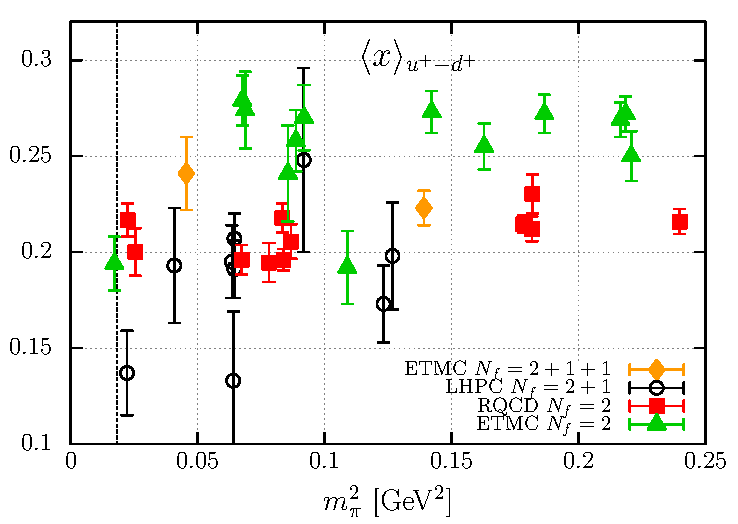
\includegraphics[width=0.4\textwidth]{plots/x_world.pdf}}
\subfloat[]{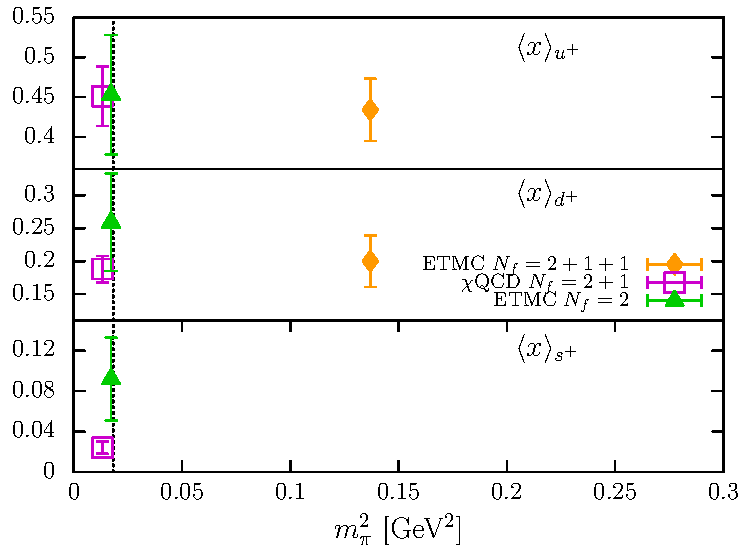
\includegraphics[width=0.38\textwidth]{plots/xq_world_ud.pdf}}
}
\centerline{
\subfloat[]{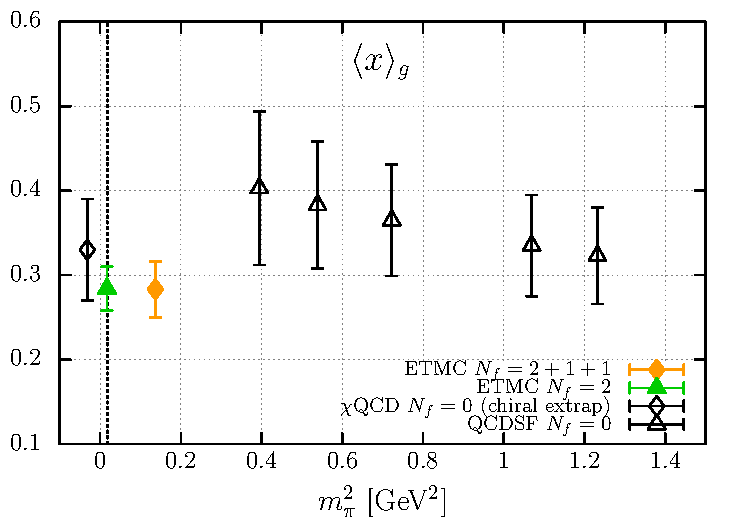
\includegraphics[width=0.4\textwidth]{plots/xg_world.pdf}}
\subfloat[]{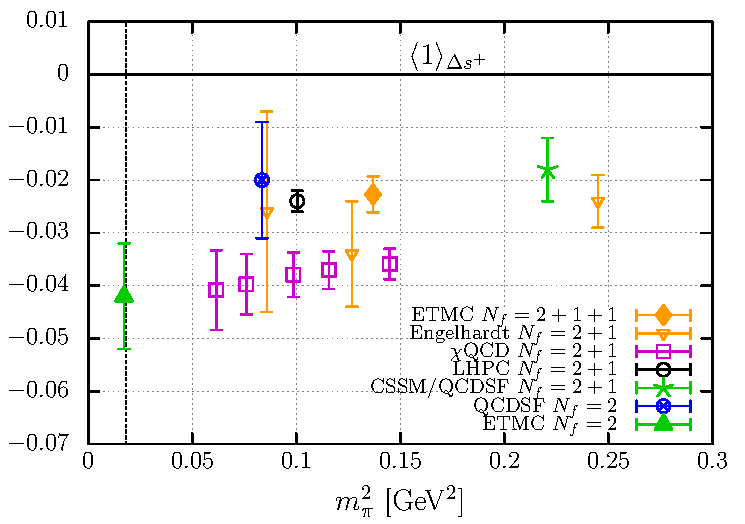
\includegraphics[width=0.4\textwidth]{plots/ga_world_strange.pdf}}
}
\centerline{
\subfloat[]{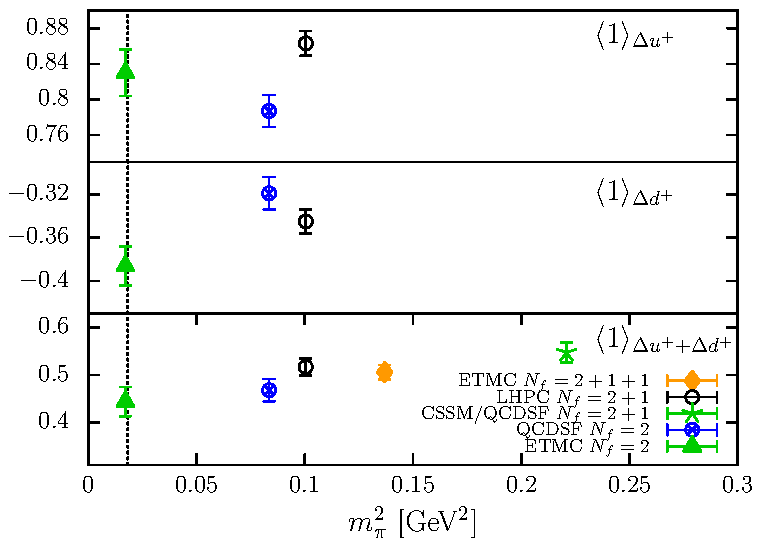
\includegraphics[width=0.4\textwidth]{plots/ga_world_ud.pdf}}
\subfloat[]{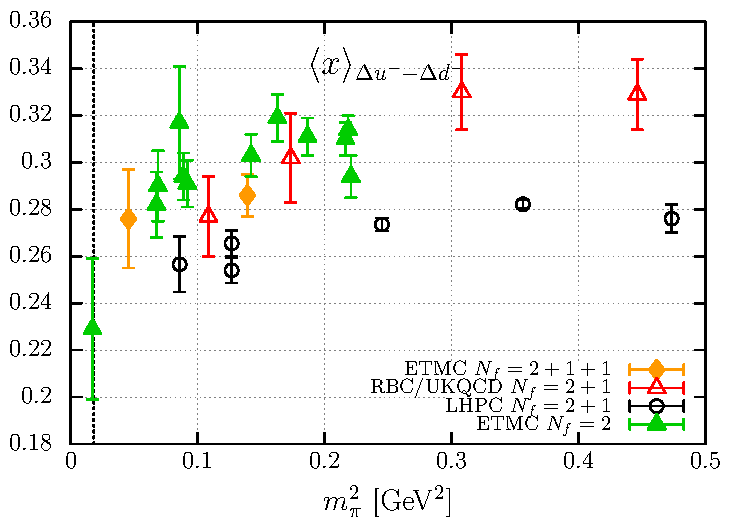
\includegraphics[width=0.4\textwidth]{plots/xdeltaq_isovector.pdf}}
}
\end{center}
\caption{Physical and unphysical pion mass results for lattice-QCD calculations of the zeroth and first moments
of unpolarised and polarised PDFs.}
\label{fig:latt_res}
\end{figure}
%%%%%%%%%%%%%%%%%%%%%%%%%%%%%%%%%%%%%%%%%%%%%%%%%%%%%%%%%%%%%%%%%%%%%



%%%%%%%%%%%%%%%%%%%%%%%%%%%%%%%%%%%%%%%%%%%%%%%%%%%%%%%%%%%%%%%%%%%%%
\begin{table}
\renewcommand{\arraystretch}{1.2} 
\centering
\makebox[\textwidth]{ % Centre table on page, even though it is a little wide
\begin{tabular}{llllll}
  Ref. & Sea quarks & Valence quarks & Renormalization & $N_{\Delta t}$ & $m_\pi$ (MeV)\\
\hline

  Mainz '17b* \cite{Capitani:2017qpc} &
  2 clover & clover & Schrödinger functional & 4--6 & 193--473\\

  ETMC '17* \cite{Alexandrou:2017hac} &
  2 clover-TM & clover-TM & Rome-Southampton & 3 & 131\\

  CalLat '17* \cite{Berkowitz:2017gql} &
  2+1+1 staggered & domain wall & Rome-Southampton & all & 131--313 \\

  LHPC '17 \cite{Green:2017keo} &
  2+1 clover & clover & Rome-Southampton & 5 & 317 \\

  NME '17 \cite{Yoon:2016jzj} &
  2+1 clover & clover & Rome-Southampton & 1**,4--5 & 172--285 \\

  Mainz '17a \cite{vonHippel:2016wid} &
  2 clover & clover & Schrödinger functional & 4--6 & 193--456\\

  Dragos et al.\ '16 \cite{Dragos:2016rtx} &
  3 clover & clover & Rome-Southampton & 1,2**,5 & 460 \\

  PNDME '16 \cite{Bhattacharya:2016zcn} &
  2+1+1 staggered & clover & Rome-Southampton & 3--5 & 128--319\\

  $\chi$QCD '16 \cite{Yang:2015zja} &
  2+1 domain wall & overlap & $Z_A/Z_V=1$ & 3 & 330 \\

  ETMC '15b \cite{Abdel-Rehim:2015owa} &
    2 clover-TM & \multicolumn{4}{l}{superseded by ETMC '17} \\
  & 2 twisted mass & twisted mass & Rome-Southampton & 1 & 262--470\\
  & 2+1+1 twisted mass & twisted mass & & 1, 4 & 213, 373\\

  RQCD '15 \cite{Bali:2014nma} &
  2 clover & clover & Rome-Southampton & 1--5 & 150--490\\

  PNDME '14 \cite{Bhattacharya:2013ehc} &
  \multicolumn{5}{l}{superseded by PNDME '16} \\

  QCDSF '14 \cite{Horsley:2013ayv} &
  2 clover & clover & $g_A/f_\pi \times f_\pi^\text{phys}$ & 1,5 & 157--1591 \\

  LHPC '14 \cite{Green:2012ud} &
  2+1 clover & clover & Rome-Southampton & 3 & 149--356\\

  ETMC '13 \cite{Alexandrou:2013joa} &
  \multicolumn{5}{l}{superseded by ETMC '15b} \\

  CSSM '13 \cite{Owen:2012ts} &
  2+1 clover & clover & Schrödinger functional & 1**$^\dagger$ & 290 \\

  Mainz '12 \cite{Capitani:2012gj} &
  \multicolumn{5}{l}{superseded by Mainz '17b} \\

  ETMC '11 \cite{Alexandrou:2011nr} &
  \multicolumn{5}{l}{superseded by ETMC '15b} \\

  LHPC '10 \cite{Bratt:2010jn} &
  2+1 staggered & domain wall & $A_\mu/\mathcal{A}_\mu$ ratio & 1--2 & 293--758 \\

  RBC+UKQCD '09 \cite{Yamazaki:2009zq} &
  2+1 domain wall & domain wall & $Z_A/Z_V=1$ & 1 & 329--668 \\

  RBC+UKQCD '08 \cite{Yamazaki:2008py} &
  \multicolumn{5}{l}{superseded by RBC+UKQCD '09} \\

  RBC '08 \cite{Lin:2008uz} &
  2 domain wall & domain wall & $Z_A/Z_V=1$ & 1--2 & 493--695 \\

  LHPC '08 \cite{Hagler:2007xi} &
  \multicolumn{5}{l}{superseded by LHPC '10} \\

  Alexandrou et al.\ '07 \cite{Alexandrou:2007xj} &
  2 Wilson & Wilson & Rome-Southampton & 1 & 384--691 \\

  LHPC '06 \cite{Edwards:2005ym} &
  \multicolumn{5}{l}{superseded by LHPC '10} \\

  QCDSF '06 \cite{Khan:2006de} &
  \multicolumn{5}{l}{superseded by QCDSF '14?} \\
\hline
\end{tabular}
} % End makebox
\begin{minipage}{\linewidth}
{\footnotesize 
\begin{itemize}
\item[$*$] Preprint.
\item[$**$] A variationally optimized interpolating operator is employed.
\item[$\dagger$] Carried out with a single fixed source-operator separation and all source-sink separations.
\end{itemize}
}
\end{minipage}
\caption{Full details of lattice-QCD calculations of the axial coupling $g_A\equiv\langle 1\rangle_{\Delta u^+-\Delta d^+}$.
We omit quenched results, perturbatively renormalized results, and conference proceedings.}
\end{table}
%%%%%%%%%%%%%%%%%%%%%%%%%%%%%%%%%%%%%%%%%%%%%%%%%%%%%%%%%%%%%%%%%%%%%


%%%%%%%%%%%%%%%%%%%%%%%%%%%%%%%%%%%%%%%%%%%%%%%%%%%%%%%%%%%%%%%%%%%%%
\begin{table}
\renewcommand{\arraystretch}{1.2} 
\centering
\makebox[\textwidth]{ % Centre table on page, even though it is a little wide
\begin{tabular}{lllll}
  Ref. & Flavours & Sea quarks & Valence quarks & Renormalization \\
\hline

  ETMC '17* \cite{Alexandrou:2017hac} &
  $u,d,s,c$ & 2 clover-TM & clover-TM & Rome-Southampton \\

  $\chi$QCD '17* \cite{Gong:2015iir} &
  $s,c$ & 2+1 domain wall & overlap & single-flavour anomalous WI \\

  LHPC '17 \cite{Green:2017keo} &
  $u,d,s$ & 2+1 clover & clover & Rome-Southampton \\

  CSSM and &
  $u+d+s$ &
  2+1, 3 clover & clover & Rome-Southampton \\
  QCDSF/UKQCD '15 \cite{Chambers:2015bka} & conn.\ / disc. & & & \\

  ETMC '14 \cite{Abdel-Rehim:2013wlz} &
  $u+d,s$ & 2+1+1 twisted mass & twisted mass & non-singlet Rome-Southampton\\

  Engelhardt '12 \cite{Engelhardt:2012gd} &
  $s$ & 2+1 staggered & domain wall & non-singlet $A_\mu/\mathcal{A}_\mu$ ratio \\

  QCDSF '12 \cite{QCDSF:2011aa} &
  $u,d,s$ & 2 clover & clover & non-singlet Rome-Southampton \\
  & & & &+ two-loop singlet-nonsinglet\\

  Babich et al.\ '10 \cite{Babich:2010at} &
  $s$ & 2 aniso-clover & aniso-clover & none \\

  SESAM '99 \cite{Gusken:1999as} &
  $u,d,s$ & 2 Wilson & Wilson & one loop \\

  $\chi$QCD '95 \cite{Dong:1995rx} &
  $u,d,s$ & quenched & Wilson & one loop \\

  Fukugita et al.\ '95 \cite{Fukugita:1994fh} &
  $u,d,s$ & quenched & Wilson & one loop \\

  Gupta and Mandula '94 \cite{Gupta:1994qw} &
  singlet** & quenched & Wilson & anomalous Ward identity \\

  Allés et al.\ '94 \cite{Alles:1994ss} &
  singlet** & quenched & Wilson & anomalous Ward identity \\

  Altmeyer et al.\ '94 \cite{Altmeyer:1992nt} &
  singlet & 4 staggered & staggered & anomalous Ward identity \\

  Mandula and Ogilvie '93 \cite{Mandula:1992bc} &
  $s$** & quenched & Wilson & none \\
  \hline
\end{tabular}
} % End makebox
\begin{minipage}{\linewidth}
{\footnotesize 
\begin{itemize}
\item[$*$] Preprint.
\item[$**$] No signal available.
\end{itemize}
}
\end{minipage}
\caption{Full details of lattice-QCD calculations of the non-isovector quark spins. Early works are summarized in Ref.~\cite{Liu:1995kb}. \emph{ADD NEW ETMC PAPER!!!!}}
\end{table}
%%%%%%%%%%%%%%%%%%%%%%%%%%%%%%%%%%%%%%%%%%%%%%%%%%%%%%%%%%%%%%%%%%%%%


%%%%%%%%%%%%%%%%%%%%%%%%%%%%%%%%%%%%%%%%%%%%%%%%%%%%%%%%%%%%%%%%%%%%%
\begin{table}
\renewcommand{\arraystretch}{1.2} 
\centering
\makebox[\textwidth]{ % Centre table on page, even though it is a little wide
\begin{tabular}{llllll}
  Ref. & Sea quarks & Valence quarks & Renormalization & $N_{\Delta t}$ & $m_\pi$ (MeV)\\
\hline

  $\chi$QCD '16 \cite{Yang:2015zja} &
  2+1 domain wall & overlap & one loop & 3 & 330 \\

  ETMC '15b \cite{Abdel-Rehim:2015owa} &
    2 clover-TM & clover-TM & Rome-Southampton & 3 & 131 \\
  & 2 twisted mass & twisted mass & & 1 & 262--470\\
  & 2+1+1 twisted mass & twisted mass & & 1, 5 & 213, 373\\

  ETMC '15a \cite{Alexandrou:2015qia} &
  2+1+1 twisted mass & twisted mass & Rome-Southampton & 1 & 302--466 \\

  RQCD '14 \cite{Bali:2014gha} &
  2 clover & clover & Rome-Southampton & 1--6 & 149--490 \\

  LHPC '14 \cite{Green:2012ud} &
  2+1 clover & clover & Rome-Southampton & 3 & 149--356\\

  ETMC '13 \cite{Alexandrou:2013joa} &
  \multicolumn{5}{l}{superseded by ETMC '15b} \\

  RQCD '12 \cite{Bali:2012av} &
  \multicolumn{5}{l}{superseded by RQCD '14} \\

  ETMC '11 \cite{Alexandrou:2011nr} &
  \multicolumn{5}{l}{superseded by ETMC '15b} \\

  QCDSF/UKQCD '11* \cite{Pleiter:2011gw} &
  2 clover & clover & Rome-Southampton & 1 & 170--670 \\

  LHPC '11* \cite{Syritsyn:2011vk} &
  2+1 domain wall & domain wall & Rome-Southampton & 1 & 297--403 \\

  LHPC '10 \cite{Bratt:2010jn} &
  2+1 staggered & domain wall & one-loop $Z_\mathcal{O}/Z_A$ & 1--2 & 293--758 \\

  RBC-UKQCD '10 \cite{Aoki:2010xg} &
  2+1 domain wall & domain wall & Rome-Southampton & 1 & 329--668 \\

  RBC '08 \cite{Lin:2008uz} &
  2 domain wall & domain wall & Rome-Southampton & 1--2 & 493--695 \\

  LHPC '08 \cite{Hagler:2007xi} &
  \multicolumn{5}{l}{superseded by LHPC '10} \\

  LHPC and &
  2 Wilson & Wilson & one loop & 1--2 & ?\\
  SESAM '02 \cite{Dolgov:2002zm} &
  and quenched & & & \\
\hline
\end{tabular}
} % End makebox
\begin{minipage}{\linewidth}
{\footnotesize 
\begin{itemize}
\item[$*$] Conference proceedings.
\end{itemize}
}
\end{minipage}
\caption{Full details of lattice-QCD calculations of the $\langle x\rangle_{u^+-d^+}$. We omit quenched and non-renormalized results.}
\end{table}
%%%%%%%%%%%%%%%%%%%%%%%%%%%%%%%%%%%%%%%%%%%%%%%%%%%%%%%%%%%%%%%%%%%%%


%%%%%%%%%%%%%%%%%%%%%%%%%%%%%%%%%%%%%%%%%%%%%%%%%%%%%%%%%%%%%%%%%%%%%
\begin{table}
\renewcommand{\arraystretch}{1.2} 
\centering
\makebox[\textwidth]{ % Centre table on page, even though it is a little wide
\begin{tabular}{lllll}
  Ref. & Flavours & Sea quarks & Valence quarks & Renormalization \\
\hline

  ETMC '16* \cite{Alexandrou:2016ekb} & $g$
    & 2+1+1 twisted mass & twisted mass & one loop \\
  & & 2 clover-TM & clover-TM & \\

  ETMC '15a \cite{Alexandrou:2015qia} &
  $u+d-2s$ &  2+1+1 twisted mass & twisted mass & Rome-Southampton \\

  ETMC '14 \cite{Abdel-Rehim:2013wlz} &
  $u+d$ & 2+1+1 twisted mass & twisted mass & non-singlet Rome-Southampton\\

  $\chi$QCD '15 \cite{Deka:2013zha} &
  $u,d,s,g$ & quenched & Wilson & sum rule + one-loop \\

  QCDSF-UKQCD '12 \cite{Horsley:2012pz} &
  $g$ & quenched & clover & nonperturbative \\
\hline
\end{tabular}
} % End makebox
\begin{minipage}{\linewidth}
{\footnotesize 
\begin{itemize}
\item[$*$] Preprint.
\end{itemize}
}
\end{minipage}
\caption{Full details of lattice-QCD calculations of the non-isovector momentum fractions. }
\end{table}
%%%%%%%%%%%%%%%%%%%%%%%%%%%%%%%%%%%%%%%%%%%%%%%%%%%%%%%%%%%%%%%%%%%%%



%%%%%%%%%%%%%%%%%%%%%%%%%%%%%%%%%%%%%%%%%%%%%%%%%%%%%%%%%%%%%%%%%%%%%
\begin{table}
\renewcommand{\arraystretch}{1.2} 
\centering
\makebox[\textwidth]{ % Centre table on page, even though it is a little wide
\begin{tabular}{lllll}
  Ref. & Sea quarks & Valence quarks & Renormalization & $N_{\Delta t}$ \\
  \hline

  ETMC '15b \cite{Abdel-Rehim:2015owa} &
    2 clover-TM & clover-TM & Rome-Southampton & 3 \\
  & 2 twisted mass & twisted mass & & 1 \\
  & 2+1+1 twisted mass & twisted mass & & 1 or 4 \\

  ETMC '13 \cite{Alexandrou:2013joa} &
  \multicolumn{4}{l}{superseded by ETMC '15b} \\

  ETMC '11 \cite{Alexandrou:2011nr} &
  \multicolumn{4}{l}{superseded by ETMC '15b} \\

  QCDSF/UKQCD '11* \cite{Pleiter:2011gw} &
  2 clover & clover & Rome-Southampton & 1 \\

  LHPC '10 \cite{Bratt:2010jn} &
  2+1 staggered & domain wall & one-loop $Z_\mathcal{O}/Z_A$ & 1--2 \\

  RBC-UKQCD '10 \cite{Aoki:2010xg} &
  2+1 domain wall & domain wall & Rome-Southampton & 1 \\

  RBC '08 \cite{Lin:2008uz} &
  2 domain wall & domain wall & Rome-Southampton & 1--2 \\

  LHPC '08 \cite{Hagler:2007xi} &
  \multicolumn{4}{l}{superseded by LHPC '10} \\

  LHPC and &
  2 Wilson & Wilson & one loop & 1--2 \\
  SESAM '02 \cite{Dolgov:2002zm} &
  and quenched & & & \\

  QCDSF '97 \cite{Gockeler:1997zr} &
  quenched & Wilson & one loop & 1 \\
\hline
\end{tabular}
} % End makebox
\begin{minipage}{\linewidth}
{\footnotesize 
\begin{itemize}
\item[$*$] Conference proceedings.
\end{itemize}
}
\end{minipage}
\caption{Full details of lattice-QCD calculations of $\langle x\rangle_{\Delta u^--\Delta d^-}$. }
\end{table}
%%%%%%%%%%%%%%%%%%%%%%%%%%%%%%%%%%%%%%%%%%%%%%%%%%%%%%%%%%%%%%%%%%%%%


%%%%%%%%%%%%%%%%%%%%%%%%%%%%%%%%%%%%%%%%%%%%%%%%%%%%%%%%%%%%%%%%%%%%%
\begin{table}
\renewcommand{\arraystretch}{1.2} 
\centering
\makebox[\textwidth]{ % Centre table on page, even though it is a little wide
\begin{tabular}{lllll}
  Ref. & Flavours & Sea quarks & Valence quarks & Renormalization \\
\hline
  ETMC '14 \cite{Abdel-Rehim:2013wlz} &
  $u+d$ & 2+1+1 twisted mass & twisted mass & non-singlet Rome-Southampton\\
  \hline
\end{tabular}
} % End makebox
\caption{Full details of lattice-QCD calculations of non-isovector polarized momentum fractions. }
\end{table}
%%%%%%%%%%%%%%%%%%%%%%%%%%%%%%%%%%%%%%%%%%%%%%%%%%%%%%%%%%%%%%%%%%%%%


%%%%%%%%%%%%%%%%%%%%%%%%%%%%%%%%%%%%%%%%%%%%%%%%%%%%%%%%%%%%%%%%%%%%%
\begin{table}
\renewcommand{\arraystretch}{1.2} 
\centering
\makebox[\textwidth]{ % Centre table on page, even though it is a little wide
\begin{tabular}{lllll}
  Ref. & Observables & Sea quarks & Valence quarks & Renormalization \\
\hline

  LHPC '10$^{\dagger}$
  \cite{Bratt:2010jn} &
  $\langle x\rangle_{u^+-d^+}$,
  $\langle x^2\rangle_{u^--d^-}$, &
  2+1 staggered &
  domain wall &
  one-loop $Z_\mathcal{O}/Z_A$ \\
  &   $g_A$,
  $\langle x\rangle_{\Delta u^--\Delta d^-}$,
  $\langle x^2\rangle_{\Delta u^+-\Delta d^+}$ & & & \\

  $\chi$QCD '09 \cite{Deka:2008xr} &
  $\langle x\rangle_{u^+,d^+,s^+}$ (superseded by $\chi$QCD '15), &
  quenched &
  Wilson &
  one loop \\
  & $\langle x^2 \rangle_{u^-,d^-,s^-}$ & & &\\

  LHPC '08 \cite{Hagler:2007xi} &
  superseded by LHPC '10 & & &\\

  QCDSF '05c \cite{Gockeler:2005vw} &
  $\langle x^2\rangle_{\Delta u^+-\Delta d^+}$ &
  2 clover & clover & Rome-Southampton \\

  QCDSF '05b \cite{Gockeler:2004wp} &
  $\langle x\rangle_{u^+-d^+}$,
  $\langle x^2\rangle_{u^--d^-}$,
  $\langle x^3\rangle_{u^+-d^+}$ &
  quenched &
  clover &
  Rome-Southampton \\

  QCDSF '05a* \cite{Gockeler:2004vx} &
  $\langle x\rangle_{u^+-d^+}$,
  $\langle x^2\rangle_{u^--d^-}$,
  $\langle x^3\rangle_{u^+-d^+}$ &
  2 clover & clover & one loop \\

  LHPC and &
  $\langle x\rangle_{u^+-d^+}$,
  $\langle x^2\rangle_{u^--d^-}$,
  $\langle x^3\rangle_{u^+-d^+}$, &
  2 Wilson & Wilson & one loop \\
  SESAM '02 \cite{Dolgov:2002zm} &
  $g_A$,
  $\langle x\rangle_{\Delta u^--\Delta d^-}$,
  $\langle x^2\rangle_{\Delta u^+-\Delta d^+}$ &
  and quenched & & \\

  QCDSF '01 \cite{Gockeler:2000ja} &
  $\langle x^2\rangle_{\Delta u^+-\Delta d^+}$ &
  quenched & clover & Rome-Southampton \\

  QCDSF '96 \cite{Gockeler:1995wg} &
  $\langle x\rangle_{u^+-d^+}$,
  $\langle x^2\rangle_{u^--d^-}$,
  $\langle x^3\rangle_{u^+-d^+}$, &
  quenched & Wilson & one loop \\
  & $g_A$,
  $\langle x^2\rangle_{\Delta u^+-\Delta d^+}$ & & &\\
\hline
\end{tabular}
} % End makebox
\begin{minipage}{\linewidth}
{\footnotesize 
\begin{itemize}
\item[$*$] Conference proceedings.
\item[$\dagger$] The moment $\langle x^2\rangle_{u-d}=A_{30}^{u-d}(0)$ is plotted in the ratio of form factors $A_{30}(t)/A_{10}(t)$, where we can use $A_{10}^{u-d}(0)=1$. The moment $\langle x^2\rangle_{\Delta u-\Delta d}=\tilde A_{30}^{u-d}(0)$ is plotted in the ratio of form factors $\tilde A_{30}(t)/\tilde A_{10}(t)$ and we can use $\tilde A_{10}^{u-d}(0)=g_A$.
\end{itemize}
}
\end{minipage}
\caption{Full details of lattice-QCD calculations of higher moments of unpolarised and polarised PDFs. }
\end{table}
%%%%%%%%%%%%%%%%%%%%%%%%%%%%%%%%%%%%%%%%%%%%%%%%%%%%%%%%%%%%%%%%%%%%%
